\section{Cubic spline}
% Cubic spline is a cubic function between two points, \(X_{i-1}\) and \(X_i\), where the function is defined in equation \ref{eq:cubic_spline}.
% \begin{equation}
%  X_{i-1, i} (t) = a_i t^3 + b_i t^2 + c_i t + d
%  \label{eq:cubic_spline}
% \end{equation}

The position to cubic spline is found using \cite[equation 5.23]{book:roboticNotes}

Then the transformation matrix is then found by using the start rotation and the new position.

Cubic spline is applied between the given points.

The inverse kinematic is then found by using the Jacobian inverse kinematic solver.

The inverse kinematic positions can be seen in table \ref{tb:positions}.

\begin{table}[h]
\centering
\begin{tabular}{l|*{3}{c} }
 time    & x      & y      & z      \\ \hline       
 t=0.50s & -0.975 & -0.502 & -0.032 \\
 t=1.05s & -0.974 & -0.435 & -0.032 \\
 t=1.32s & -0.979 & -0.450 & -0.032 \\
 t=1.70s & -0.902 & -0.450 & -0.032 \\
\end{tabular}
\caption{Positions during the movement.}
\label{tb:positions}
\end{table}

The joint positions is found and shown in table \ref{tb:joint_positions}.

\begin{table}[h]
\centering
\begin{tabular}{l|*{6}{c} }
 time    & q(0)   & q(1)   & q(2)  & q(3)   & q(4)  & q(5)   \\ \hline       
 t=0.50s & -0.066 & -0.815 & 1.349 & -0.534 & 1.505 & -1.571 \\
 t=1.05s & -0.762 & -0.427 & 0.596 & -0.170 & 0.809 & -1.571 \\
 t=1.32s & -0.751 & -0.415 & 0.572 & -0.157 & 0.820 & -1.571 \\
 t=1.70s & -0.963 & -0.826 & 1.370 & -0.543 & 0.608 & -1.571 \\
\end{tabular}
\caption{Positions during the movement.}
\label{tb:joint_positions}
\end{table}

The positions is printed to a lua script\cite{zip:luaScript}.

Velocity constraints is applied and the tau is calculated and plotted in figure \ref{fig:tau_v_t}.

\begin{figure}
 \centering
 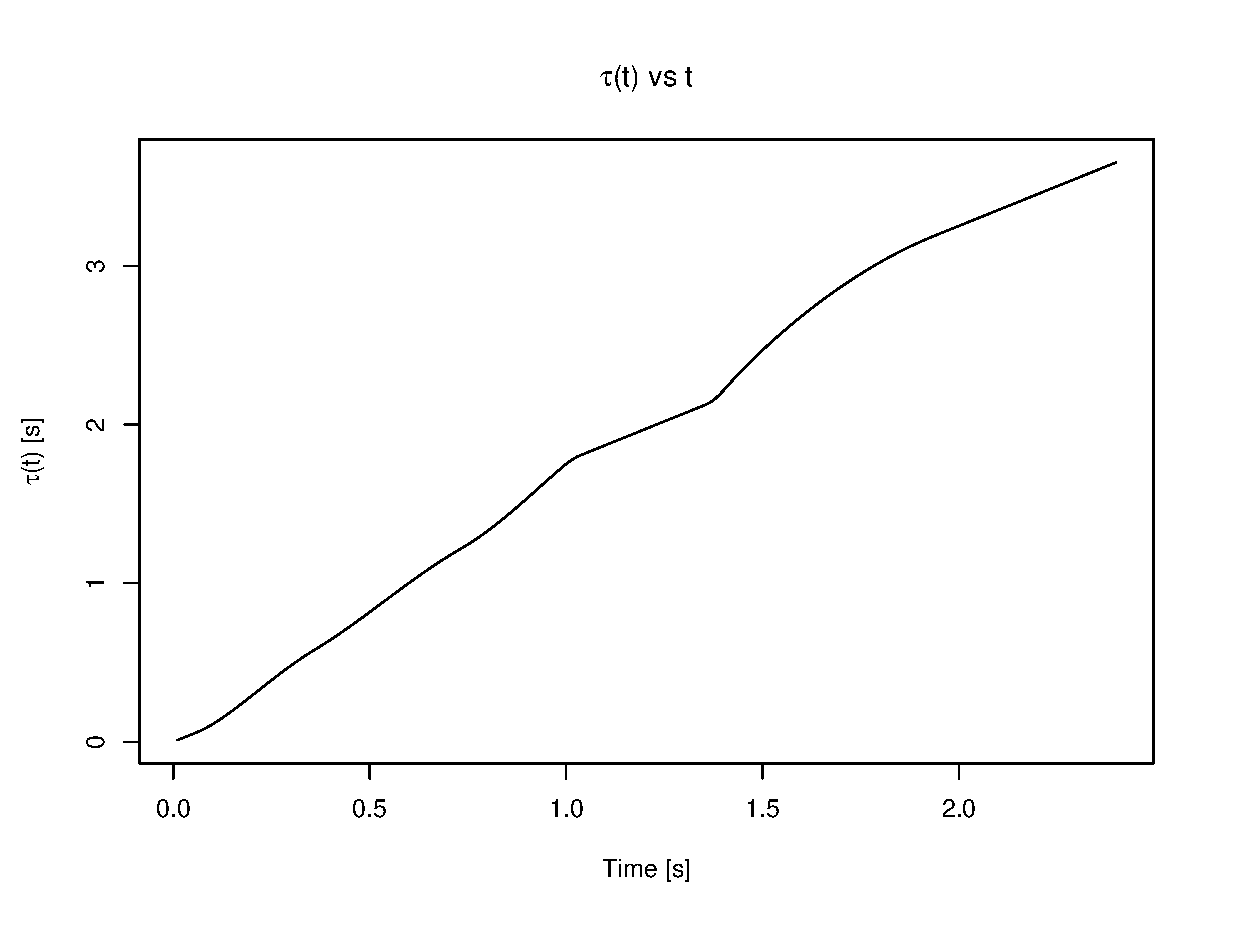
\includegraphics[width=0.7\linewidth]{graphics/timeplot}
 \caption{$\tau(t)$ vs t.}
 \label{fig:tau_v_t}
\end{figure}
